\section{Results}
    \subsection{Classification}
        % Table with the one best accuracy score from the two methods
        % Figure with analysis of regularization parameters and learning rates
		Following are the results for the SGD algorithm applied to the credit card data set. Table \ref{tab:sgdresults} lists the accomplishment of the SGD accuracy:
		\begin{table}[H]
			\centering
			\begin{tabular}[t]{lcccc} % @{\hskip 0.4in}
				\toprule
				- & Epochs & Batchsize & Learning Rate &
				\bottomrule
			\end{tabular}
			\caption{Table listing the accuracy result of the SGD algorithm.}
			\label{tab:sgdresults}
		\end{table}
		These results were produced using the following parameters:
		\begin{itemize}
			\item Batchsize = 100
			\item Test percentage = $33\%$
			\item Hidden layers: []
		\end{itemize}
		
		
		
		
		
	
		NN_epochs = 100
		
		learning_rate = 0.1
		
		regularization_param = 0         # set lambda = 0, eta = 0.01
		
		Following are the results from the ANN study of the credit card data. The accuracy scores of the neural network hyperparameter and learning rate grid search are illustrated in figure \ref{fig:cc_acc}.
		\begin{figure}[H]
			\centering
			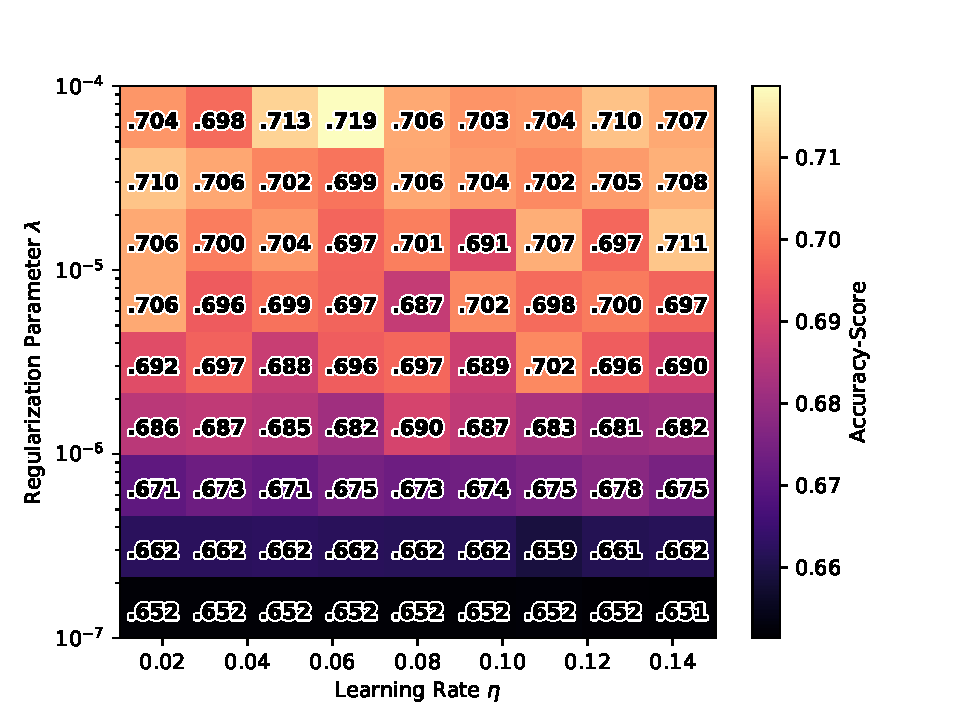
\includegraphics[width=0.45\textwidth]{figures/cc_res_0.pdf}
			\caption{The accuracy score of the classification neural network for different $\eta$ and $\lambda$ values. The maximum accuracy score of the array is $0.719$, using $\eta=0.056$ and $\lambda=10^{-4}$}
			\label{fig:cc_acc}
		\end{figure}
		The F1-scores of the neural network hyperparameter and learning rate grid search are illustrated in figure \ref{fig:cc_F1}.
		\begin{figure}[H]
			\centering
			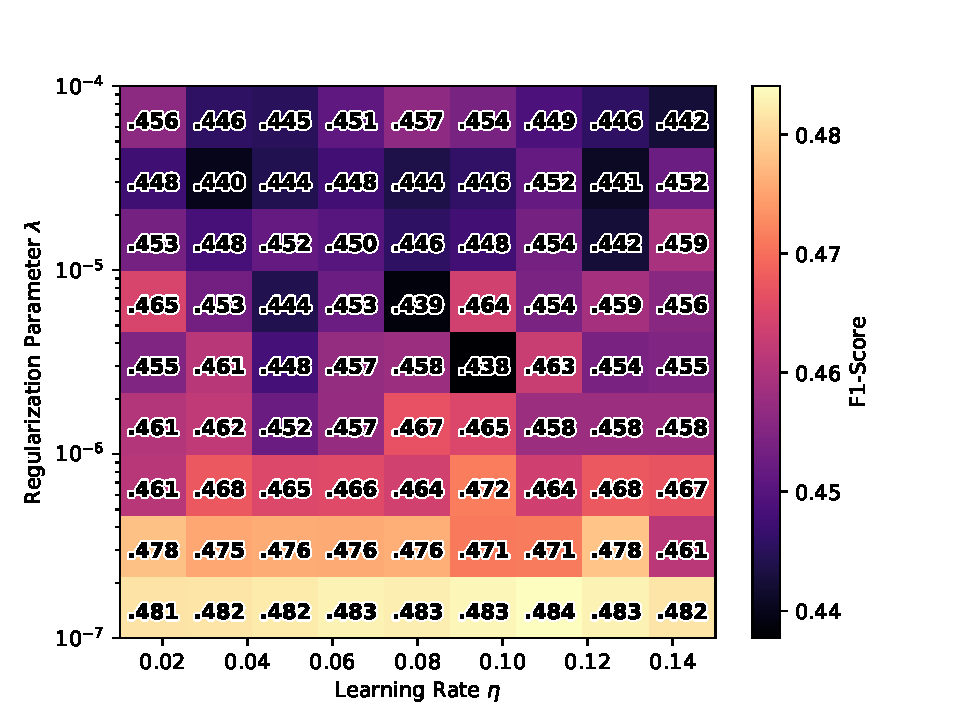
\includegraphics[width=0.45\textwidth]{figures/cc_res_1.pdf}
			\caption{The F1 score of the classification neural network for different $\eta$ and $\lambda$ values. The maximum F1 score of the array is $0.484$, using $\eta=0.103$ and $\lambda=10^{-7}$}
			\label{fig:cc_F1}
		\end{figure}
		The AUC-scores of the neural network hyperparameter and learning rate grid search are illustrated in figure \ref{fig:cc_auc}.
		\begin{figure}[H]
			\centering
			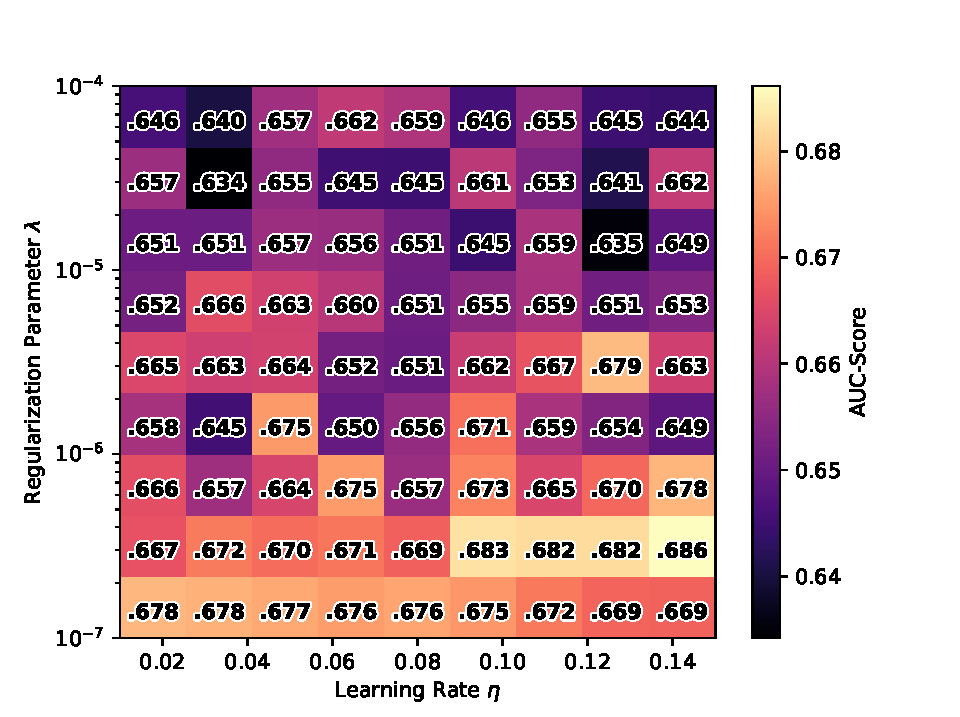
\includegraphics[width=0.45\textwidth]{figures/cc_res_2.pdf}
			\caption{The AUC-score of the classification neural network for different $\eta$ and $\lambda$ values. The maximum AUC-score of the array is $0.686$, using $\eta=0.150$ and $\lambda=2.154\cdot 10^{-7}$}
			\label{fig:cc_auc}
		\end{figure}
		The gains-ratio of the neural network hyperparameter and learning rate grid search are illustrated in figure \ref{fig:cc_gr}.
		\begin{figure}[H]
			\centering
			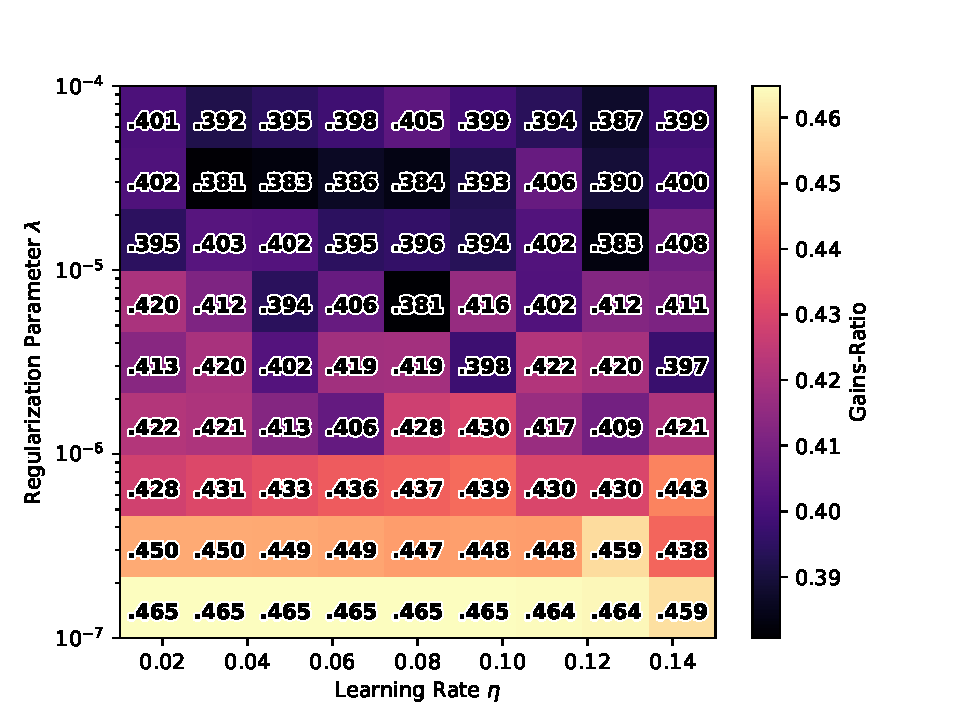
\includegraphics[width=0.45\textwidth]{figures/cc_res_3.pdf}
			\caption{The gains-ratio of the classification neural network for different $\eta$ and $\lambda$ values. The maximum gains-ratio of the array is $0.465$, using $\eta \in [0.010, 0.103]$ and $\lambda=10^{-7}$}
			\label{fig:cc_gr}
		\end{figure}
	
        
        
    \subsection{Regression}
    
    	The mean squared error and the $R^2$-score of the regression neural network for different $\eta$ and $\lambda$-values after studing Franke's function can be seen in figure \ref{fig:ff_mse} and \ref{fig:ff_r2} respectively.
    
    	\begin{figure}[H]
    		\centering
    		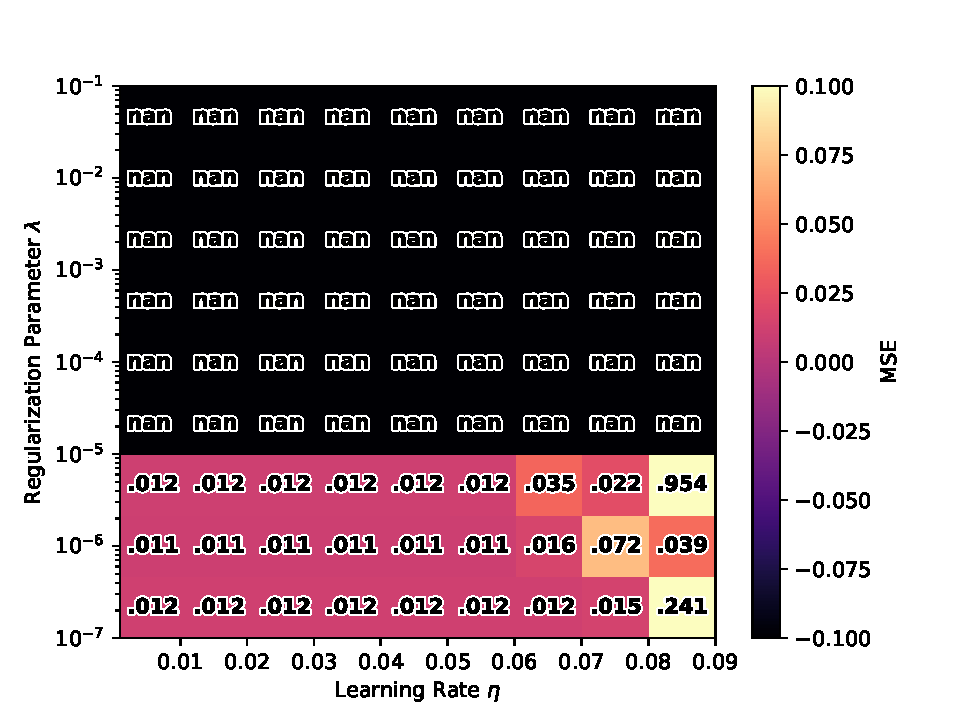
\includegraphics[width=0.45\textwidth]{figures/ff_res_0.pdf}
    		\caption{The mean squared error of the regression neural network for different $\eta$ and $\lambda$-values after studing Franke's function.}
    		\label{fig:ff_mse}
    	\end{figure}
    	\begin{figure}[H]
    		\centering
    		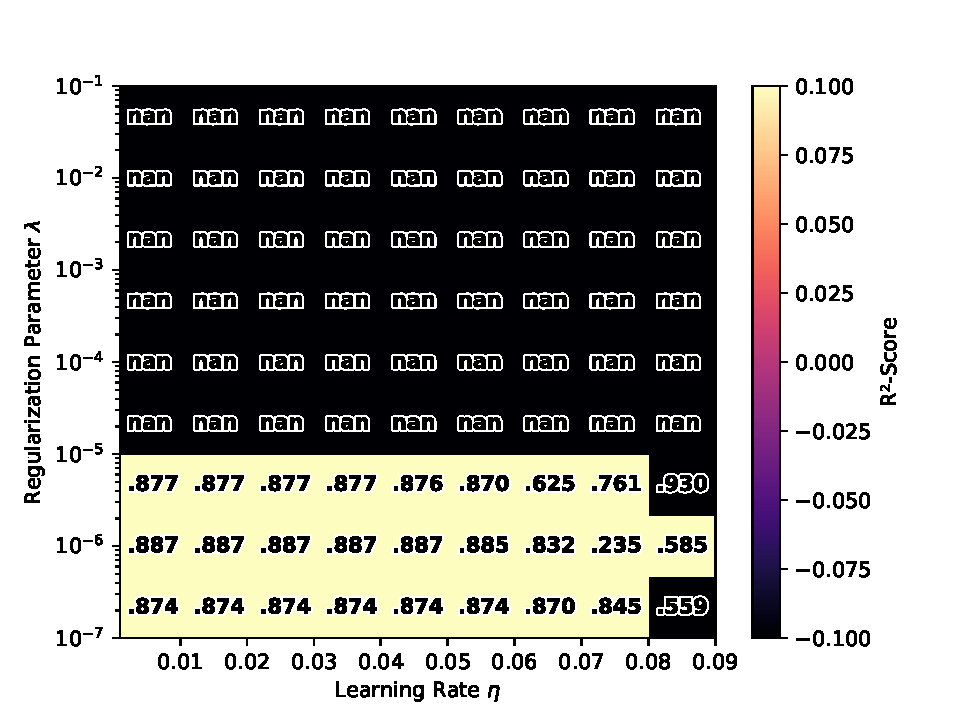
\includegraphics[width=0.45\textwidth]{figures/ff_res_1.pdf}
    		\caption{The $R^2$-score of the regression neural network after studing Franke's function.}
    		\label{fig:ff_r2}
    	\end{figure}
    
    
    	
%        Following is a table from project 1, listing the precision of three regression schemes applied to Franke's function:
%        \begin{table}[H]
%            \centering
%            \caption{Table listing the final results and comparisons of the regressional methods applied to Franke's function with $n=10,000$ data points.}
%            \begin{tabular}[t]{l@{\hskip 0.3in}c@{\hskip 0.3in}c@{\hskip 0.2in}c}
%                \toprule
%                Scheme & MSE minimum & $p_{deg}$ & $\log(\lambda)$ \\
%                \midrule
%                OLS & 0.2493 & 8 & $-$\\
%                Ridge & 0.2489 & 11 & -9\\
%                Lasso & 0.2524 & 8 & -12\\
%                \bottomrule
%            \end{tabular}
%            \label{tab:conclusion_table_Frankes}
%        \end{table}
%        
%        
%        \begin{figure}[H]
%            \centering
%            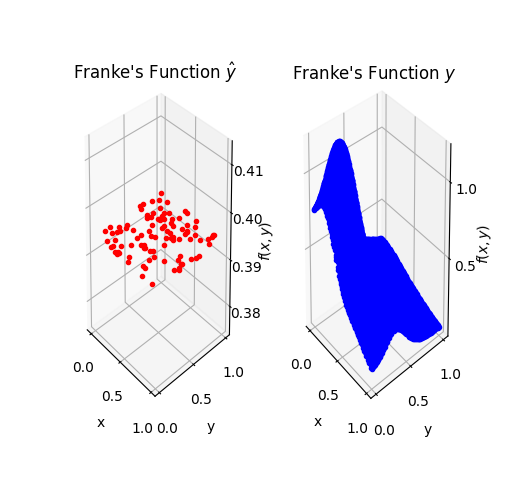
\includegraphics[width=0.4\textwidth]{figures/regression_NNW.png}
%            \caption{The ANN regression on Franke's function. With $MSE=4.08$.}
%            \label{fig:ANNREG}
%        \end{figure}
        
        
        % Table with the least MSE from the two methods
        % (Figure with analysis of regularization parameters and learning rates): this is not specifically asked for in the problem set, it wants: a discussion of reg. params./learning rates